\chapter{Důkazy}\label{chap:dukazy}
V matematice se lze setkat s celou řadou různých tvrzení. Od primitivních, jejichž platnost je zřejmá až po složitější, nad jejich platností je třeba se více zamyslet. Čtenář se nejspíše zatím spíše setkával s matematikou, která zahrnovala užívání jistých postupů. Např. zjednodušování algebraických výrazů, řešení soustav rovnic, ověřování trigonometrických identit, aj. Avšak hodně postupů v matematice je založeno na již známých výsledcích, o nichž bylo dokázáno, že jsou pravdivé. Pokud ovšem máme dokázat určité tvrzení, je třeba, aby bylo naše zdůvodnění jednoznačné a logicky správné. V této sekci se proto podíváme na důkazové techniky používané v matematice, které budeme dále v textu využívat.\par
Matematická tvrzení jsou často různě klasifikována v závislosti na jejich povaze. Základními typy jsou tyto. 
\begin{itemize}
    \item \emph{Axiom}. Tvrzení, které implicitně považujeme za pravdivé a nedokazujeme jej. S axiomatikou jsme se již částečně seznámili v historické předmluvě (viz \ref{subsec:tm_soucasnost}).
    \item \emph{Věta}. Matematické tvrzení, jehož pravdivost můžeme ověřit důkazem.
    \item \emph{Lemma}. Pomocné tvrzení, které běžně využíváme pro důkaz jiného (typicky složitějšího) tvrzení.
    \item \emph{Důsledek}. Tvrzení, které je přímým důsledkem jiného tvrzení.
\end{itemize}
Čistě formálně však mezi \textbf{větou}, \textbf{lemmatem} a \textbf{důsledkem} není žádný rozdíl.

\section{Důkaz přímý}\label{sec:dukaz_primy}
Jedná se o asi nejjednodušší typ důkazu. Často jsou matematická tvrzení formulována jako implikace, tzn. "Jestliže platí $A$, pak platí $B$.". Konkrétně, např. "Je-li $x<0$, pak $x^2>0$.".\par
Myšlenka důkazu je taková, že začínáme od předpokladu $A$, z něhož dále odvozujeme dílčí tvrzení tak dlouho, až dojdeme k požadovanému závěru $B$. Symbolicky, pokud si označíme dílčí tvrzení v důkazu $X_1, X_2, \dots, X_n$, pak vlastně dokazujeme výrokovou formuli
\begin{equation}\label{eq:primy_dukaz_formule}
    (A \implies X_1) \land (X_1 \implies X_2) \land \cdots \land (X_{n-1}\implies X_n) \land (X_n \implies B).
\end{equation}
V tomto procesu dokazování se využívá tautologie \ref{item:tautologie_4} z věty \ref{thm:vyznamne_tautologie}
\begin{equation*}
    (A \implies B) \land (B \implies C) \iff (A \implies C).
\end{equation*}
Z tohoto faktu vyplývá, že pokud je každá z dílčích implikací pravdivá, pak je nutně pravdivá i implikace $A \implies B$, kterou jsme chtěli dokázat\footnote{Výrokové proměnné lze v konkrétním případě nahradit příslušnými predikáty.}. Podívejme se na příklad podobný příklad z úvodu.

\begin{proposition}
    Nechť $x\in\R$. Je-li $x<0$, pak $x^2+1>0$.
\end{proposition}
\begin{proof}
    Předpokladem našeho tvrzení je $x\in\R \land x<0$. Víme, že pro každé reálné číslo $x$ platí, že $x^2\geq 0$. Tj. určitě platí implikace
    \begin{equation*}
        x<0 \implies x^2>0.
    \end{equation*}
    Dále víme, že triviálně platí $1>0$, tedy také jistě platí
    \begin{equation*}
        x^2+1>x^2.
    \end{equation*}
    Protože však $x^2>0$, pak také
    $x^2+1>0$, což jsme chtěli dokázat.
\end{proof}
Posloupnost dokázaných implikací bychom mohli podle \eqref{eq:primy_dukaz_formule} zapsat nyní jako
\begin{equation*}
    (x\in\R \land x<0 \implies x^2>0) \land (x^2>0 \implies x^2+1>x^2) \land (x^2+1>x^2 \implies x^2+1>0),
\end{equation*}
a tedy jsme dokázali i implikaci v původním tvrzení $x<0 \implies x^2+1>0$.\par
V praxi důkazy takto samozřejmě nerozepisujeme a řadu věcí považujeme za samozřejmé, např. právě $1>0$, $x^2+1>x^2$, apod. Takový důkaz bychom bez většího rozepisování mohli napsat klidně na jeden řádek.
\begin{equation*}
    x<0 \implies 0<x^2<x^2+1 \implies x^2+1>0.
\end{equation*}
Všimněte si zároveň, že jsme zde použili jistou generalizaci. Předvedený důkaz totiž není závislý na volbě $x$ a náš argument je tak univerzální. Tedy platí
\begin{equation*}
    \forall x<0: x^2+1>0.
\end{equation*}
Obecně tvrzení formulovaná stylem "je-li $x\in X$, pak \dots" jsou míněna jako
\begin{equation*}
    \forall x\in X: \dots
\end{equation*}
\begin{proposition}
    Nechť $n\in\N$ je liché. Pak $3n+7$ je sudé číslo.
\end{proposition}
\begin{proof}
    Začneme u předpokladu, že $n\in\N$ je liché číslo. To znamená, že
    \begin{equation*}
        \exists k\in\N : n=2k+1.
    \end{equation*}
    Po dosazení obdržíme
    \begin{equation*}
        3(2k+1)+7=6k+3+7=6k+10=2(3k+5).
    \end{equation*}
    Protože $3k+5$ je přirozené číslo, pak $3n+7$ je dělitelné dvěma a je tedy sudé, což jsme chtěli dokázat.
\end{proof}
\begin{proposition}[AG nerovnost]
    Pro $a,b\in\R_0^+$ platí
    \begin{equation*}
        \sqrt{ab}\leq\dfrac{a+b}{2}.
    \end{equation*}
\end{proposition}
\begin{proof}
    Při důkazu tohoto tvrzení vyjdeme z jednoduchého pozorování:
    \begin{equation*}
        (\sqrt{a}+\sqrt{b})^2\geq 0.
    \end{equation*}
    Nyní stačí výraz upravit a dostaneme požadovanou nerovnost.
    \begin{equation*}
        (\sqrt{a}+\sqrt{b})^2 = a+2\sqrt{ab}+b\geq 0 \implies \sqrt{ab}\leq \dfrac{a+b}{2}.
    \end{equation*}
\end{proof}
\begin{proposition}
    Pro $\forall x,y\in\R$ platí
    \begin{equation*}
        x<y \implies x<\dfrac{x+y}{2}<y.
    \end{equation*}
\end{proposition}
\begin{proof}
    Zde je třeba si všimnout "dvojité" nerovnosti v dokazovaném tvrzení. To nám již napovídá, že ve skutečnosti musíme dokázat 2 dílčí tvrzení, konkrétně
    \begin{equation*}
        x < \dfrac{x+y}{2}\quad\text{a}\quad\dfrac{x+y}{2} < y.
    \end{equation*}
    Při důkazu obou částí vyjdeme opět z předpokladu. Tedy mějme libovolná čísla $x,y\in\R$ taková, že $x<y$. Pak jistě platí
    \begin{equation*}
        x+x<x+y \implies 2x<x+y \implies x<\dfrac{x+y}{2}.
    \end{equation*}
    Tím jsme dokázali první nerovnost. Platnost druhé dokážeme analogicky:
    \begin{equation*}
        x+y<y+y \implies x+y<2y \implies \dfrac{x+y}{2}<y.
    \end{equation*}
\end{proof}
(Převzato z \cite{ChartrandPolimeniZhang2014}, str. 79 a \cite{MatematickaLogikaUK2010}, sekce \emph{důkaz přímý}.)\\
Ne všechna tvrzení jsou v matematice nutně formulována jako implikace. Často se lze setkat s tvrzeními formulovanými jako ekvivalence, tj. $A \iff B$. Důkazy takových výroků jsou již trochu delší, neboť už nestačí pouze ukázat $A \implies B$. Vzpomeňme si však na tautologii, která nám dávala do souvislosti ekvivalenci s implikací (viz \ref{item:tautologie_2} ve větě \ref{thm:vyznamne_tautologie}):
\begin{equation*}
    (A \iff B) \iff (A \implies B) \land (B \implies A).
\end{equation*}
Z toho je již vidět, jak u takových tvrzení při důkazu postupovat. Zkrátka dokážeme zvlášť $A \implies B$ a $A \impliedby B$.
\begin{proposition}
    Nechť $x,y\in\Z$. Pak $3 \mid xy$ právě tehdy, když $3 \mid x$ nebo $3 \mid y$.
\end{proposition}
\begin{proof}
    \textit{($\implies$)}. Začneme s předpokladem, že $3 \mid xy$. Víme, že pokud je číslo dělitelné třemi, pak jej lze zapsat jako $3k$, kde $k\in\Z$. Uvažujme následující případy:
    \begin{itemize}
        \item $3 \mid x \land 3 \mid y$. Tehdy tvrzení jistě platí.
        \item $3 \nmid x$. Ukážeme, že pak nutně musí platit $3 \mid y$. Pokud $x$ není dělitelné třemi, pak jej lze zapsat buď jako $3k+1$, nebo $3k+2$, kde $k\in\Z$. 
        \begin{equation*}
            xy=(3k+1)y\quad\text{nebo}\quad xy=(3k+2)y
        \end{equation*}
        Protože čísla $3k+1$ a $3k+2$ nejsou dělitelná třemi, pak je vidět, že musí platit $3 \mid y$.
        \item $3 \nmid y$. Zde je postup analogický. 
    \end{itemize}
    Tím máme dokázanou implikaci $3 \mid xy \implies 3 \mid x \lor 3 \mid y$.\\
    \textit{($\impliedby$)}. Nyní předpokládáme, že platí $3 \mid x \lor 3 \mid y$; chceme ukázat, že $3 \mid xy$ Bez újmy na obecnosti\footnote{Termín \emph{bez újmy na obecnosti} (někdy zkráceně \emph{BÚNO}) se v matematických textech používá v situacích, kdy může nastat více možností, avšak říkáme, že jejich důkazy jsou analogické.}, nechť je $x$ dělitelné třemi. Pak existuje $x=3k$, kde $k\in\Z$. Po dosazení dostaneme
    \begin{equation*}
        xy=(3k)y=3(ky) \implies 3 \mid xy.
    \end{equation*}
    Tedy dokázali jsme obě implikace a tím i původní tvrzení.
\end{proof}

\section{Důkaz nepřímý}\label{sec:dukaz_neprimy}
Řada tvrzení v matematice však není až tak jednoduchá na dokázání přímo. Důkazy, které jsme si ukazovali, vždy začínaly od předpokladu a postupně jsme došli k požadovanému závěru. Lze ale postupovat i jinak. Opět se odkážeme na dříve zmíněné tautologie věty \ref{thm:vyznamne_tautologie}, konkrétně na \ref{item:tautologie_5}:
\begin{equation}\label{eq:dukaz_neprimy_tautologie}
    (A \implies B) \iff (\neg B \implies \neg A).
\end{equation}
Implikace je ve skutečnosti ekvivalentní s tvrzením, že pokud neplatí závěr, pak neplatí ani předpoklad. Na této skutečnosti je založen \emph{důkaz nepřímý} (též \emph{důkaz obměnou}). Podívejme se na příklady užití.
\begin{proposition}
    Nechť $x\in\Z$ a $3 \nmid (x^2-1)$. Pak $3 \mid x$.
\end{proposition}
V tomto případě máme dvě možnosti. Buď začneme s předpokladem $3 \nmid (x^2-1)$~a dokážeme, že $3 \mid x$ (tedy dokážeme tvrzení přímo), nebo naopak budeme předpokládat, že $3 \nmid x$ a dokážeme negaci původního předpokladu. Ačkoliv by se jistě našla možnost, jak tvrzení dokázat přímo, přesto se nejspíše zdá jednodušší začít s předpokladem, že $x$ není dělitelné třemi.
\begin{proof}
    Nechť $3 \nmid x$. Ukážeme, že platí $3 \mid (x^2-1)$. Podle předpokladu lze $x$ zapsat jako $3k+1$ nebo $3k+2$, kde $k\in\Z$. Bez újmy na obecnosti pišme $x=3k+1$. Pak
    \begin{equation*}
        x^2-1=(3k+1)^2-1=9k^2+6k+1-1=9k^2+6k=3(3k^2+2k)\implies 3 \mid (x^2-1).
    \end{equation*}
    Tedy dokázali jsme, že
    \begin{equation*}
        3 \nmid x \implies 3 \mid (x^2-1),
    \end{equation*}
    což je však podle \ref{eq:dukaz_neprimy_tautologie} ekvivalentní s
    \begin{equation*}
        3 \nmid (x^2-1) \implies 3 \mid x
    \end{equation*}
    a původní tvrzení je tak dokázané.
\end{proof}
\begin{proposition}
    Nechť jsou dány množiny $A$ a $B$. Pak
    \begin{equation*}
        A \cup B=A \iff B \subseteq A.
    \end{equation*}
\end{proposition}
\begin{proof}
    \textit{($\implies$)}. Tuto implikaci dokážeme obměnou. Nechť jsou dány množiny $A$ a $B$ takové, že $B$ není podmnožinou $A$. Pak
    \begin{equation*}
        \exists x\in B : x\notin A.
    \end{equation*}
    Prvek $x$ se se tedy objeví i ve sjednocení $A \cup B$, tj.
    \begin{equation*}
        x\in A \cup B.
    \end{equation*}
    Ale protože $x\notin A$, pak $A \cup B \neq A$.\\
    \textit{($\impliedby$)}. Opačnou implikaci lze již dokázat přímo a využijeme zde poměrně hezkého triku, který se při dokazování podobných tvrzení využívá. Tvrdíme-li, že dvě množiny se rovnají, pak ovšem i platí, že jsou vzájemně podmnožinami té druhé. Symbolicky
    \begin{equation*}
        X = Y \iff (X \subseteq Y) \land (Y \subseteq X).
    \end{equation*}
    V našem případě budeme chtít ukázat, že platí
    \begin{equation*}
        (A \subseteq A \cup B) \land (A \cup B \subseteq A).
    \end{equation*}
    Platnost inkluze $A \subseteq A \cup B$ je vidět okamžitě (vyplývá z definice sjednocení), neboť pro libovolný prvek $x$ platí:
    \begin{equation*}
        x \in A \implies x \in A \cup B
    \end{equation*}
    a tedy skutečně $A \subseteq A \cup B$.\par
    Zbývá ukázat, že $A \cup B \subseteq A$. Vezměme libovolný prvek $x \in A \cup B$; ukážeme že $x\in A$. Nyní mohou nastat dvě možnosti:
    \begin{itemize}
        \item $x \in A$. Pak máme triviálně požadovaný výsledek.
        \item $x \in B$. Z předpokladu víme, že $B \subseteq A$, z čehož opět plyne $x\in A$.
    \end{itemize}
    Dokázali jsme tedy obě inkluze, tj. $A \subseteq A \cup B$ a $A \cup B \subseteq A$ a tedy platí
    \begin{equation*}
        A \cup B = A.
    \end{equation*}
\end{proof}
(Převzato z \cite{ChartrandPolimeniZhang2014}, str. 111.)
\section{Důkaz sporem}\label{sec:dukaz_sporem}
Už jsme si představili dvě základní důkazové techniky. Nyní k nim přidáme metodu třetí -- \emph{důkaz sporem}.\par
Uvažme, že máme tvrzení ve tvaru implikace $A \implies B$, které chceme dokázat. Podle \ref{item:reductio_ad_absurdum} ve větě \ref{thm:vyznamne_tautologie} víme, že vždy platí
\begin{equation}\label{eq:dukaz_sporem_logika}
    (P \implies \neg P) \implies \neg P.
\end{equation}
Tato tautologie říká, že pokud z výroku $P$ lze odvodit jeho negaci $\neg P$, pak výrok $P$ neplatí.\par
Myšlenka důkazu sporem je tedy taková, že \textbf{budeme předpokládat platnost negace dokazovaného tvrzení $\neg (A \implies B)$ a dojdeme k závěru, který je v rozporu předpokladem}. Z toho pak podle \eqref{eq:dukaz_sporem_logika} plyne, že znegované tvrzení neplatí a podle \emph{zákona vyloučeného třetího} (viz \ref{item:zakon_vylouceneho_tretiho} ve větě \ref{thm:vyznamne_tautologie}) musí platit tvrzení opačné (což je původní tvrzení).\par
Ještě si vzpomeňme na tautologii
\begin{equation*}
    (A \implies B) \iff B \lor \neg A.
\end{equation*}
Pomocí ní můžeme psát
\begin{equation*}
    \neg (A \implies B) \equiv \neg (B \lor \neg A) \equiv A \land \neg B.
\end{equation*}
To ostatně dává i smysl. Implikace je nepravdivá pouze, když platí její předpoklad, ale neplatí její závěr.
\begin{proposition}
    Nechť jsou dána $a,b\in\Z$, kde $a$ je sudé a $b$ je liché. Pak\linebreak $4 \nmid (a^2+2b^2)$.
\end{proposition}
\begin{proof}
    Nejprve znegujeme dokazované tvrzení, tj.
    \begin{equation*}
        \neg \bigl((2 \mid a \land 2 \nmid b) \implies 4 \nmid (a^2+2b^2)\bigr) \iff (2 \mid a \land 2 \nmid b) \land 4 \mid (a^2+2b^2).
    \end{equation*}
    Pro spor tedy předpokládejme, že je-li $a$ sudé a $b$ liché, pak výraz $a^2+2b^2$ je dělitelný čtyřmi. Tedy existují čísla $k,l\in\Z$ taková, že $a=2k$ a $b=2l-1$. Tedy
    \begin{equation*}
        a^2+2b^2=(2k)^2+2(2l-1)^2=4k^2+8l^2-8l+2=4(k^2+2l^2-2l)+2.
    \end{equation*}
    Výraz $4(k^2+2l^2-2l)$ je jistě dělitelný 4. Avšak protože platí $4 \mid a^2+2b^2$, pak musí také platit $4 \mid 2$. To očividně však neplatí. To znamená, že znegované tvrzení je nepravdivé a platí tvrzení původní, což jsme chtěli dokázat.
\end{proof}
(Převzato z \cite{ChartrandPolimeniZhang2014}, str. 126)
V případě důkazu sporem je asi nejznámější (a též i nejstarší dochovaný) důkaz, že číslo $\sqrt{2}$ je iracionální.
\begin{proposition}
    Číslo $\sqrt{2}$ je iracionální.
\end{proposition}
\begin{proof}
    Než začneme s důkazem, trochu si rozmysleme dokazované tvrzení. Jak bude vypadat jeho negace? Opačným tvrzením je, že \emph{číslo $\sqrt{2}$ je racionální}. Z~definice racionálního čísla to však znamená
    \begin{equation*}
        \exists p,q\in\Z : \sqrt{2}=\dfrac{p}{q}.
    \end{equation*}
    O každém zlomku však víme, že jej lze zapsat v základním tvaru, tj. můžeme zároveň předpokládat, že $p$ a $q$ jsou nesoudělná. S tímto budeme dále pracovat. Pišme
    \begin{align*}
        \sqrt{2}&=\dfrac{p}{q}\\
        2&=\dfrac{p^2}{q^2}\\
        2q^2&=p^2.
    \end{align*}
    Z posledního řádku lze vidět, že $p^2$ lze zapsat jako dvojnásobek nějakého jiného čísla. Tedy $p^2$ je určitě sudé. Co nám to říká o samotném $p$? Že $p$ je také sudé. (O tom není těžké se přesvědčit. Stačí si spočítat $(2k)^2$ a analogicky pro lichá čísla $(2l-1)^2$.) Tzn. že existuje $r\in\Z$ takové, že $p=2r$. Nyní dosadíme:
    \begin{align*}
        2q^2&=(2r)^2\\
        2q^2&=4r^2\\
        q^2&=2r^2.
    \end{align*}
    Tedy $q^2$ je také nutně sudé a tedy i $q$ je sudé. Dohromady tedy $p$ a $q$ jsou obě sudá. To je však spor, neboť jsme předpokládali, že $p$ a $q$ jsou nesoudělná. Tzn. nemůže neexistovat zlomek $p/q$, který by byl roven $\sqrt{2}$ a byl v základním tvaru.
\end{proof}
\begin{proposition}\label{prop:prvocisla}
    Prvočísel je nekonečně mnoho.
\end{proposition}
\begin{proof}
    Pro spor naopak uvažujme, že prvočísel je konečně mnoho; označme si je $p_1, p_2, \dots, p_n$. Definujeme číslo $m$ následovně:
    \begin{equation*}
        m=p_1p_2\cdots p_n.
    \end{equation*}
    Nyní k číslu $m$ přičteme 1
    \begin{equation*}
        m+1=p_1p_2\cdots p_n+1.
    \end{equation*}
    Na závěr celou rovnost vydělíme kterýmkoliv z čísel $p_1, p_2, \dots, p_n$; bez újmy na obecnosti zvolme $p_1$:
    \begin{equation*}
        \dfrac{m+1}{p_1}=\dfrac{p_1p_2\cdots p_n+1}{p_1}=p_2\cdots p_n+\dfrac{1}{p_1}.
    \end{equation*}
    Číslo $p_2\cdots p_n$ je jistě přirozené, avšak $1/p_1$ již přirozené není (nejmenší prvočíslo je 2). Je vidět, že nově vzniklé přirozené číslo $m+1$ není dělitelné žádným z prvočísel $p_1, p_2, \dots, p_n$. To však znamená, že $m+1$ je buď samo prvočíslo, nebo je dělitelné prvočíslem, které není součástí posloupnosti $p_1, p_2, \dots, p_n$. V obou případech však dostáváme spor, neboť jsme předpokládali, že posloupnost $p_1, p_2, \dots, p_n$ obsahuje všechna prvočísla.
\end{proof}

\section{Důkaz matematickou indukcí}\label{sec:dukaz_indukci}
K této důkazové technice si na úvod ukažme příklad. Čtenáři je jistě znám vzorec pro součet prvních $n$ členů geometrické posloupnosti. Jistě tak pro nás neměl být problém určit součet
\begin{equation*}
    \sum_{k=0}^{n}{2^k}.
\end{equation*}
Představme si na chvíli, že bychom neznali daný vzorec. Zkusme si vypočítat prvních několik hodnot:
\begin{align*}
    2^0&=1,\\
    2^0+2^1&=3,\\
    2^0+2^1+2^2&=7,\\
    2^0+2^1+2^2+2^3&=15.
\end{align*}
Zdá se, že vzorec pro obecné $n$ by mohl být $2^{n+1}-1$. Ale i kdybychom to ověřili pro jakékoliv množství hodnot $n$, stále to nebude není důkaz. Jak na to? K podobným tvrzením se využívá tzv. \emph{matematická indukce} (někdy zkráceně jen \emph{indukce}). Ukažme si na tomto příkladu způsob použití (formální princip si vysvětlíme později).\par
Naším cílem je tedy dokázat, že $\forall n\in\N_0$ platí
\begin{equation*}
    \sum_{k=0}^{n}{2^k}=2^{n+1}-1.
\end{equation*}
\begin{enumerate}[label=(\roman*)]
    \item\label{item:zaklad_indukce} Nejdříve ověříme platnost vzorce pro nejmenší možné $n$, tj. pro $n=0$:
    \begin{equation*}
        \sum_{k=0}^{0}{2^k}=2^0=1\quad\text{a}\quad2^{0+1}-1=2-1=1.
    \end{equation*}
    Pro $n=0$ vzorec platí.
    \item\label{item:indukcni_krok} Nyní předpokládejme, že tvrzení platí pro určité $n=n_0\in\N$. Ukážeme, že pak tvrzení nutně musí platit i pro $n=n_0+1$. Pišme
    \begin{equation*}
        \sum_{k=0}^{n_0+1}{2^k}=\sum_{k=0}^{n_0}{2^k}+2^{n_0+1}.
    \end{equation*}
    Podle předpokladu vzorec platí pro $n_0$, tedy za $\sum_{k=0}^{n_0}{2^k}$ můžeme dosadit $2^{n_0+1}-1$. Tedy
    \begin{equation*}
        \sum_{k=0}^{n_0}{2^k}+2^{n_0+1}=2^{n_0+1}-1+2^{n_0+1}=2\cdot 2^{n_0+1}-1=2^{n_0+2}-1.
    \end{equation*}
    To je ale přesně vzorec pro $n=n_0+1$.
\end{enumerate}
Tím jsme dokázali dané tvrzení. Jak? Podle \ref{item:zaklad_indukce} vzorec platí pro $n=0$. Podle \ref{item:indukcni_krok} pak platí, že když tvrzení platí pro $n=0$, pak platí i pro $n=1$ (pro $n_0=0$). Pro $n=1$ pak opět podle \ref{item:indukcni_krok} platí, že tvrzení platí i pro $n=2$. Opět podle \ref{item:indukcni_krok} víme, že když tvrzení platí pro $n=2$, pak platí i pro $n=3$ a tak dále. Z~tohoto principu plyne, že tvrzení tedy platí pro všechna $n\in\N$ (viz obrázek \ref{fig:domino}).
\begin{figure}[H]
    \centering
    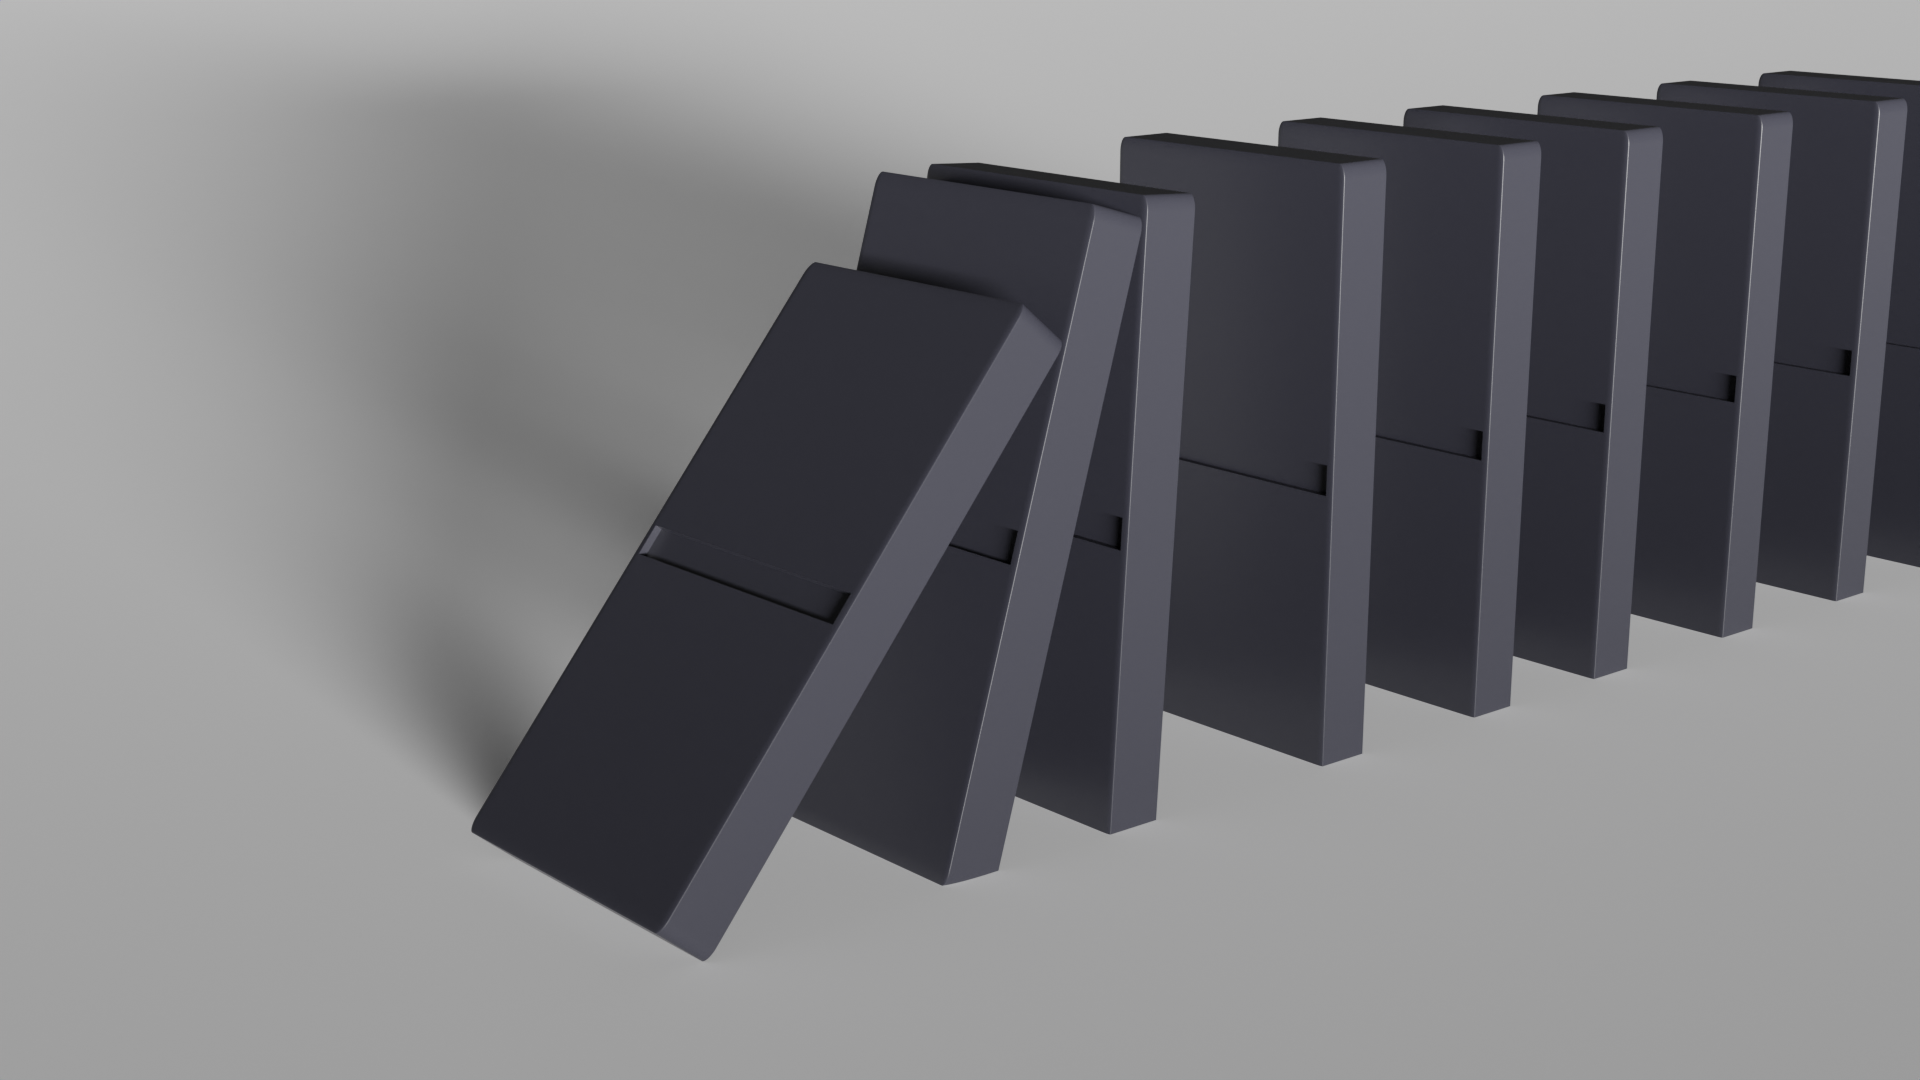
\includegraphics[scale=\fullhd]{ch02_domino_indukce.png}
    \caption{Důkaz indukcí lze přirovnat k efektu padajícího domina.}
    \label{fig:domino}
\end{figure}
Krok \ref{item:indukcni_krok} se nazývá \emph{indukční krok} a předpoklad, že dokazované tvrzení platí pro nějaké $n=n_0$ se nazývá \emph{indukční předpoklad}. Někdy se v důkazech indukcí pro upřesnění specifikuje, podle jaké proměnné dané tvrzení dokazujeme. V tomto případě bychom řekli \emph{"indukcí podle $n$"}. (Inspirováno \cite{MatousekNesetril2009}, str. 32.)\\
Tento postup vychází z tzv. \emph{principu matematické indukce}, který lze zformulovat jako větu.
\begin{theorem}[Princip matematické indukce]
    Nechť pro každé $n\in\N$ je $\varphi_n$ libovolný výrok. Pokud platí
    \begin{enumerate}[label=(\roman*)]
        \item $\varphi_1$ a
        \item $\forall k\in\N: \varphi_k \implies \varphi_{k+1}$,
    \end{enumerate}
    pak platí $\forall n\in\N: \varphi_n$.
\end{theorem}
(Převzato z \cite{ChartrandPolimeniZhang2014}, str. 144.)\\
Tuto větu v různých textech lze najít i v jiných formulacích. Její důkaz však vyžaduje složitější znalosti. Uveďme si ještě jeden příklad.
\begin{convention}
    Při aplikaci indukčního předpokladu se někdy píše zkratka \emph{I.~P.}, čehož se budeme držet v dalším textu.
\end{convention}
\begin{proposition}
    Pro každé přirozené $n\geq 5$ platí $2^n>n^2$.
\end{proposition}
\begin{proof}
    Tvrzení dokážeme indukcí podle $n$.
    \begin{itemize}
        \item Pro nejmenší hodnotu $n=5$ dostáváme $2^5=32>5^2=25$, což jistě platí.
        \item Nyní dokážeme indukční krok. Předpokládejme, že tvrzení platí pro libovolné $n_0\geq 5$; ukážeme platnost pro $n_0+1$:
        \begin{equation*}
            2^{n_0+1}=2^{n_0}\cdot 2\stackrel{\text{I. P.}}{>} n_0^2 \cdot 2.
        \end{equation*}
        Pro dokázání tvrzení nyní stačí ukázat, že $2n_0^2 > (n_0+1)^2$.
        \begin{align*}
            2n_0^2 &= n_0^2+n_0^2>n_0^2+5n_0=n_0^2+2n_0+3n_0=n_0^2+2n_0+15\\
            &>n_0^2+2n_0+1=(n_0+1)^2.
        \end{align*}
        Celkově tedy dostáváme $2^{n_0+1}>(n_0+1)^2$.
    \end{itemize}
    Podle principu matematické indukce platí $\forall n\geq 5: 2^n>n^2$, což jsme chtěli dokázat.
\end{proof}
(Převzato z \cite{ChartrandPolimeniZhang2014}, str. 153.)
% V sekci \ref{sec:mnoziny_a_cisla} o množinách a číslech jsme si slíbili, že si dokážeme tvrzení o mohutnosti potenční množiny libovolné konečné množiny. Existuje více způsobů, jak platnost tohoto tvrzení dokázat (hodně z nich jsou více kombinatorického charakteru). My si jej však dokážeme indukcí pomocí poměrně hezkého triku.
\begin{proposition}
    Nechť $X$ je libovolná $n$-prvková množina. Pak $\sizeof{\powset{X}}=2^n$.
\end{proposition}
\begin{proof}
    Postupujme indukcí podle mohutnosti $n$ množiny $X$. Pro $n=0$ obsahuje potenční množina množiny $X$ pouze prázdnou množinu, tj. $\sizeof{\powset{\emptyset}}=2^0=1$.\par
    Předpokládejme, že tvrzení platí pro množinu o $n_0$ prvcích. Pro důkaz indukčního kroku mějme množinu $X$ o $n_0+1$. Vezměme libovolný prvek $x \in X$. Prvky potenční množiny $\powset{X}$ si rozdělíme do množin $T$ a $T^\prime$ takto:
    \begin{itemize}
        \item $T=\set{Q \in \powset{X} \admid x\in Q}$ a
        \item $T^\prime=\set{Q \in \powset{X} \admid x\notin Q}$.
    \end{itemize}
    Tedy v $T$ se nachází všechny podmnožiny množiny $X$ obsahující prvek $x$ a v $T^\prime$ všechny podmnožiny, které jej neobsahují. Z definice lze vidět, že $T$ a $T^\prime$ jsou disjunktní, tj. $T \cap T^\prime=\emptyset$ a tedy $X=T\cup T^\prime$. Jaké jsou mohutnosti $T$ a $T^\prime$? Množina $T^\prime$ obsahuje všechny podmnožiny množiny $X\setminus\set{x}$ a tedy podle indukčního předpokladu má $2^{n_0}$ podmnožin, tj. $\sizeof{\powset{X\setminus\set{x}}}=2^{n_0}$.\par
    Jak vypadají množiny obsažené v $T$? Uvažme libovolnou podmnožinu $A^\prime$ množiny $X$, která neobsahuje prvek $x$. Taková množina musí být (z definice) prvkem množiny $T^\prime$. Pokud nyní položíme množinu $A=A^\prime\cup \set{x}$, získáme tak množinu obsahující prvek $x$ a tudíž $A\in T$. Naopak pokud bychom měli množinu $B$ obsahující prvek $x$, tj. $B\in A$, pak definováním $B^\prime=B\setminus \set{x}$ získáme množinu z $T^\prime$. To však znamená, že každé množině $A^\prime\in T^\prime$ odpovídá právě jedna množina $A\in T$.\par
    Z toho plyne, že počet množin v $T$ je stejný\footnote{Formálně vzato jsme sestrojili \emph{bijekci} mezi množinami $T$ a $T^\prime$, kde obrazem množiny $A\in T$ je $A\setminus \set{x}\in T^\prime$. Termín je zaveden v sekci \ref{sec:zobrazeni}.} jako v $T^\prime$, tj. $\sizeof{T}=\sizeof{T^\prime}$, což podle již aplikovaného indukčního předpokladu znamená, že $\sizeof{T}=2^{n_0}$. Protože však množiny $T$ a $T^\prime$ jsou disjunktní, pak celkový počet prvků je $2^{n_0}+2^{n_0}=2^{n_0+1}$, což jsme chtěli dokázat.
\end{proof}